\documentclass[docid=2018/19]{tcom_exam}
\begin{document}
\setcounter{chapter}{17}
\exam{Exam 2018/19}
{
\renewcommand{\thesubsubsection}{\thesubsection\alph{subsubsection}}
\subsection{Group I}
\questionitem{Item a}
\begin{minipage}[c]{0.50\textwidth}
	The methodology should follow these lines:
	\begin{enumerate}
		\item Design an automaton that recognises strings of even length.
		\item Design an automaton that recognizes strings ending in 11.
		\item Join the two automata using a single initial state with $\varepsilon$-transitions to each of the automata
	\end{enumerate}
	\begin{center}
		\begin{tabular}{r | c c c}
			$\delta_N$           & 0            & 1            & $\varepsilon$ \\ \hline
			$\rightarrow q_0   $ & $\emptyset $ & $\emptyset $ & $\{q_{00}, q_{10}\}$ \\
			$         ^* q_{00}$ & $\{q_{01}\}$ & $\{q_{01}\}$ & $\emptyset$ \\
			$            q_{01}$ & $\{q_{00}\}$ & $\{q_{00}\}$ & $\emptyset$ \\
			$            q_{10}$ & $\{q_{10}\}$ & $\{q_{11}\}$ & $\emptyset$ \\
			$            q_{11}$ & $\{q_{10}\}$ & $\{q_{12}\}$ & $\emptyset$ \\
			$         ^* q_{12}$ & $\{q_{10}\}$ & $\{q_{12}\}$ & $\emptyset$
		\end{tabular}
	\end{center}
\end{minipage}
\begin{minipage}[c]{0.49\textwidth}
	\begin{center}
		\begin{tikzpicture}[->,>=stealth',node distance=2.3cm,initial text=$ $,]
			\node[state, initial			] (q0) {$q_0$};
			\node[state, accepting,above right of=q0	] (q00) {$q_{00}$};
			\node[state, right of=q00		] (q01) {$q_{01}$};
			\node[state, below right of=q0	] (q10) {$q_{10}$};
			\node[state, right of=q10		] (q11) {$q_{11}$};
			\node[state, accepting,right of=q11		] (q12) {$q_{12}$};

			\draw	(q0)	edge[left				] node{$\varepsilon$} (q00)
					(q0)	edge[left				] node{$\varepsilon$} (q10)

					(q00)	edge[bend right,below	] node{$0,1$} (q01)
					(q01)	edge[bend right,above	] node{$0,1$} (q00)

					(q10)	edge[loop below			] node{$0$} (q10)
					(q10)	edge[above				] node{$1$} (q11)

					(q11)	edge[above				] node{$1$} (q12)
					(q11)	edge[bend left,below	] node{$1$} (q10)

					(q12)	edge[loop below			] node{$1$} (q12)
					(q12)	edge[bend right,above	] node{$1$} (q10)
					;
		\end{tikzpicture}
	\end{center}
\end{minipage}
\questionitem{Item b}
\begin{minipage}[c]{0.49\textwidth}
	\begin{alignat*}{2}
		&\varepsilon close(q_0    && )=\{q_0,q_{00},q_{10}\}\\
		&\varepsilon close(q_{00} && )=\{q_{00}\}\\
		&\varepsilon close(q_{01} && )=\{q_{01}\}\\
		&\varepsilon close(q_{10} && )=\{q_{10}\}\\
		&\varepsilon close(q_{11} && )=\{q_{11}\}\\
		&\varepsilon close(q_{12} && )=\{q_{12}\}\\
	\end{alignat*}
\end{minipage}
\begin{minipage}[c]{0.49\textwidth}
	\begin{center}
		\begin{tabular}{r | c c}
			$\delta_D$                              & 0            & 1           \\ \hline
			$\rightarrow ^* \{q_0,q_{00},q_{10}\} $ & $\{q_{01},q_{10}\}$ & $\{q_{01},q_{11}\}$ \\
			$            ^* \{q_{00},q_{10}     \}$ & $\{q_{01},q_{10}\}$ & $\{q_{01},q_{11}\}$ \\
			$            ^* \{q_{00},q_{11}     \}$ & $\{q_{01},q_{10}\}$ & $\{q_{01},q_{12}\}$ \\
			$            ^* \{q_{00},q_{12}     \}$ & $\{q_{01},q_{10}\}$ & $\{q_{01},q_{12}\}$ \\
			$               \{q_{01},q_{10}     \}$ & $\{q_{00},q_{10}\}$ & $\{q_{00},q_{11}\}$ \\
			$               \{q_{01},q_{11}     \}$ & $\{q_{00},q_{10}\}$ & $\{q_{00},q_{12}\}$ \\
			$            ^* \{q_{01},q_{12}     \}$ & $\{q_{00},q_{10}\}$ & $\{q_{00},q_{12}\}$
		\end{tabular}
	\end{center}
\end{minipage}
\begin{center}
	\begin{tikzpicture}[->,>=stealth',node distance=3cm,initial text=$ $,]
		\node[state, accepting,initial,align=center				] (q0_q00_q10) {$q_0$\\$q_{00}$\\$q_{10}$};
		\node[state, right of=q0_q00_q10,align=center			] (q01_q11) {$q_{01}$\\$q_{11}$};
		\node[state, above of=q01_q11,align=center				] (q01_q10) {$q_{01}$\\$q_{10}$};
		\node[state, accepting,below of=q01_q11,align=center	] (q01_q12) {$q_{01}$\\$q_{12}$};
		\node[state, accepting,right of=q01_q10,align=center	] (q00_q10) {$q_{00}$\\$q_{10}$};
		\node[state, accepting,right of=q01_q11,align=center	] (q00_q11) {$q_{00}$\\$q_{11}$};
		\node[state, accepting,right of=q01_q12,align=center	] (q00_q12) {$q_{00}$\\$q_{12}$};

		\draw	(q0_q00_q10)	edge[left		] node{$0$} (q01_q10)
				(q0_q00_q10)	edge[above		] node{$1$} (q01_q11)

				(q00_q10)		edge[bend left=10,below] node{$0$} (q01_q10)
				(q00_q10)		edge[bend left=10] node{$1$} (q01_q11)

				(q00_q11)		edge[bend left=10] node{$0$} (q01_q10)
				(q00_q11)		edge[bend left=10] node{$1$} (q01_q12)

				(q00_q12)		edge[right		 ] node{$0$} (q01_q10)
				(q00_q12)		edge[bend left=10,below] node{$1$} (q01_q12)

				(q01_q10)		edge[bend left=10,above] node{$0$} (q00_q10)
				(q01_q10)		edge[bend left=10] node{$1$} (q00_q11)

				(q01_q11)		edge[bend left=10] node{$0$} (q00_q10)
				(q01_q11)		edge[bend right=10] node{$1$} (q00_q12)

				(q01_q12)		edge[left		 ] node{$0$} (q00_q10)
				(q01_q12)		edge[bend left=10,above] node{$1$} (q00_q12)
		 		;
	\end{tikzpicture}
\end{center}
\pagebreak
\questionitem{Item c}
From the DFA for $L_1$, $D_1$, we will find an NFA for $L_2$, $N_2$, by considering the same states and following these rules:
\begin{itemize}
	\item The initial state of $N_2$ is a state with a name different from that of any state of $D_1$; say it's $i$.
	\item If $q \in Q_{D_1}$ is an initial state, $q \in Q_{N_2}$ is a final state.
	\item If $q \in Q_{D_1}$ is a final state, then $q \in \delta_{N_2}(i,\varepsilon)$ (there exists an $\varepsilon$-transition from $r$ to $q$).
	\item If $\delta_{D_1}(q,a)=r$, then $q \in \delta_{N_2}(r,a)$ (swap direction of transitions).
\end{itemize}
Finally, convert $N_2$ to a DFA.\par
This technique allows to easily create a DFA that accepts the reverse of all strings for which we already have a DFA.
\questionitem{Item d}
\begin{center}
	\begin{tabular}{c c c}
		\begin{tikzpicture}[->,>=stealth',node distance=2.5cm,initial text=$ $,]
			\node[state, accepting,initial	] (1) {$1$};
			\node[state, accepting, below right of=1	] (3) {$3$};
			\node[state, above right of=3	] (2) {$2$};
			\draw	(1)	edge[above		] node{$a,b$} (2)
					(2)	edge[loop above	] node{$a$} (2)
					(2)	edge[bend right, left	] node{$b$} (3)
					(3)	edge[bend right, right	] node{$b$} (2)
					(3)	edge[left				] node{$a$} (1);
		\end{tikzpicture} &
		\begin{tikzpicture}[->,>=stealth',node distance=2.5cm,initial text=$ $,]
			\node[state, accepting,initial	] (1) {$1$};
			\node[state, accepting, below right of=1	] (3) {$3$};
			\node[state, above right of=3	] (2) {$2$};
			\draw	(1)	edge[above		] node{$a+b$} (2)
					(2)	edge[loop above	] node{$a$} (2)
					(2)	edge[bend right, left	] node{$b$} (3)
					(3)	edge[bend right, right	] node{$b$} (2)
					(3)	edge[left				] node{$a$} (1);
		\end{tikzpicture} &
		\begin{tikzpicture}[->,>=stealth',node distance=2.5cm,initial text=$ $,]
			\node[state, accepting,initial	] (1) {$1$};
			\node[state, accepting, right of=1	] (3) {$3$};
			\draw	(1)	edge[bend right, below	] node{$(a+b)a^*b$} (3)
					(3)	edge[bend right, above	] node{$a$} (1)
					(3) edge[loop above			] node{$ba^*b$} (3);
		\end{tikzpicture}
	\end{tabular}
\end{center}
\begin{center}
	\begin{tabular}{c | c}
		\begin{tikzpicture}[->,>=stealth',node distance=2.5cm,initial text=$ $,]
			\node[state, accepting,initial	] (1) {$1$};
			\node[state, right of=1			] (3) {$3$};
			\draw	(1)	edge[bend right, below	] node{$(a+b)a^*b$} (3)
					(3)	edge[bend right, above	] node{$a$} (1)
					(3) edge[loop above			] node{$ba^*b$} (3);
		\end{tikzpicture} &
		\begin{tikzpicture}[->,>=stealth',node distance=2.5cm,initial text=$ $,]
			\node[state, initial	] (1) {$1$};
			\node[state, accepting, right of=1	] (3) {$3$};
			\draw	(1)	edge[bend right, below	] node{$(a+b)a^*b$} (3)
					(3)	edge[bend right, above	] node{$a$} (1)
					(3) edge[loop above			] node{$ba^*b$} (3);
		\end{tikzpicture}
		\\
		\begin{tikzpicture}[->,>=stealth',node distance=2.5cm,initial text=$ $,]
			\node[state, accepting,initial	] (1) {$1$};
			\draw	(1) edge[loop above			] node{$(a+b)a^*b(ba^*b)^*a$} (1);
		\end{tikzpicture} & \\
		$((a+b)a^*b(ba^*b)^*a)^*$ & $((a+b)a^*b(ba^*b)^*a)^*(a+b)a^*b$
	\end{tabular}
\end{center}
\begin{alignat*}{12}
	((a+b)a^*b(ba^*b)^*a)^* + ((a+b)a^*b(ba^*)^*a)^*(a+b)a^*b
	&= ((a+b)a^*b(ba^*b)^*a)^*(\varepsilon+(a+b)a^*b)
\end{alignat*}
\pagebreak
\questionitem{Item e}
\begin{center}
	\begin{tabular}{c c}
		\begin{tabular}{r | c c}
			$\delta_N$        & $a$           & $b$ \\ \hline
			$\rightarrow q_0$ & $\{q_0,q_1\}$ & $\emptyset$ \\
			$         ^* q_1$ & $\emptyset$ & $\{q_0\}$
		\end{tabular} &
		\begin{tabular}{r | c c}
			$\delta_D$            & $a$           & $b$ \\ \hline
			$          \emptyset    $ & $\emptyset  $ & $\emptyset$ \\
			$\rightarrow \{q_0    \}$ & $\{q_0,q_1\}$ & $\emptyset$ \\
			$         ^* \{q_0,q_1\}$ & $\{q_0,q_1\}$ & $\{q_0\}$
		\end{tabular}
	\end{tabular}
\end{center}
\questionitem{Item f}
\begin{minipage}[c]{0.58\textwidth}
	$\{q_0,q_1\}$ is distinguishable from $\emptyset$ and $\{q_0\}$, given the first state is final, and the last two states are not final.\par
	Also, $\{q_0\}$ and $\emptyset$ are distinguishable, because for them to be indistinguishable it was required that $\emptyset$ and $\{q_0,q_1\}$ were undistinguishable (which is not true).
	\begin{center}
		\begin{tabular}{r || p{15mm} | p{15mm} | p{15mm}}
							& $\emptyset$ & $\{q_0\}$ & $^* \{q_0,q_1\}$ \\ \hline \hline
			$\emptyset$      & \cellcolor{gray}  & \cellcolor{gray}  &\cellcolor{gray} \\ \hline
			$\rightarrow \{q_0\}$        & X & \cellcolor{gray}  &\cellcolor{gray} \\ \hline
			$^* \{q_0,q_1\}$ & X & X & \cellcolor{gray}
		\end{tabular}
	\end{center}
\end{minipage}
\begin{minipage}[c]{0.4\textwidth}
	\begin{center}
		\begin{tikzpicture}[->,>=stealth',node distance=2.5cm,initial text=$ $,]
			\node[state, initial					] (q0) {$q_0$};
			\node[state, below right of=q0					] (e) {$\emptyset$};
			\node[state, accepting,above right of=e,align=center	] (q0_q1) {$q_0$\\$q_1$};
			

			\draw	(e)  edge[loop below	] node{$a,b$} (e)
					(q0) edge[bend left, above			] node{$a$} (q0_q1)
					(q0) edge[left			] node{$b$} (e)
					(q0_q1) edge[loop above] node{$a$} (q0_q1)
					(q0_q1) edge[bend left, above] node{$b$} (q0);
		\end{tikzpicture}
	\end{center}
\end{minipage}
\subsection{Group II}
\questionitem{Item a}
\begin{theorem}
	Given $L_1=\{a^n b^n \mid n \geq 0\}$ is a non-regular language, $L_2=\{0^n 1^m 2^{n-m} \mid  n \geq m \geq 0\}$ is also a non-regular language.
\end{theorem}
\begin{proof}
	Assume by absurd that $L_2$ is a regular language. We know that regular languages are closed to homomorphism. Thus, by defininf $L_1=h(L_2)$ where:
	\begin{alignat*}{2}
		h \colon \{0,1,2\} &\rightarrow \{a,b\}\\
		0                  &\mapsto a\\
		1                  &\mapsto b\\
		2                  &\mapsto b
	\end{alignat*}
	we are implying that $L_1$ is also a regular language. We thus arrive at a contradiction with the statement of the theorem, thus proving the theorem correct.
\end{proof}
\questionitem{Item b}
Regular languages are closed under the symmetric difference operator, given there is an algorithm to find the regular expression of the symmetric difference of two languages given by regular expressions.\par
Let $L_1$, $L_2$ be the regular languages for which we have regular expressions.
\begin{enumerate}
	\item Convert the two regular expressions to DFAs, $D_1$ and $D_2$.
	\item Obtain $D=D_1 \times D_2$, the cartesian product of $D_1$ and $D_2$, where a state $(q_1,q_2)\in Q_D$ (where $q_1 \in Q_{D_1}$ and $q_2 \in Q_{D_2}$) is final if exactly one of $q_1$ or $q_2$ are final states of their respective original DFAs. Thus, we are accepting strings that are accepted either by $L_1$ or by $L_2$, but not by both.
	\item Convert $D$ to a regular expression.
\end{enumerate}
We thus arrive at a regular expression of the symmetric difference of two languages.
\pagebreak
\subsection{Group III}
\begin{alignat*}{2}
	L=\{a^n w w^R a^j \mid n \geq 0, n \leq j \leq 2n, w \in \{a,b\}^*\}
\end{alignat*}
\questionitem{Item a}
\begin{alignat*}{2}
	S &\rightarrow aSa\mid aSaa\mid W\\
	W &\rightarrow aWa\mid bWb\mid \varepsilon
\end{alignat*}
\questionitem{Item b}
\begin{minipage}[c]{0.68\textwidth}
	\begin{alignat*}{12}
		S \implies aSa \implies aaSaa \implies aaWaa \implies aabWbaa \implies aabbaa
	\end{alignat*}
\end{minipage}
\begin{minipage}[c]{0.3\textwidth}
	\begin{center}
		\begin{tikzpicture}
			\Tree	[.S
						a
						[.S
							a
							[.S
								[.W
									b
									[.W $\varepsilon$ ]
									b
								]
							]
							a
						]
						a
					]
		\end{tikzpicture}
	\end{center}
\end{minipage}
\questionitem{Item c}
Yes it is ambiguous, given string $aabbaa$ has at least two different syntax trees: the one presented in the previous item, and the following syntax tree.
\begin{center}
	\begin{tikzpicture}
		\Tree	[.S
					a
					[.S
						[.W
							a
							[.W
								b
								[.W $\varepsilon$ ]
								b
							]
							a
						]
					]
					a
				]
	\end{tikzpicture}
\end{center}
An equivalent, non-ambiguous grammar is:
\begin{alignat*}{2}
	S &\rightarrow aSaa\mid W\\
	W &\rightarrow aWa\mid bWb\mid \varepsilon
\end{alignat*}
\questionitem{Item d}
\begin{minipage}[c]{0.49\textwidth}
	\begin{equation*}
		PDA~P=(\{q\},\{a,b\},\{a,b,S,T,W,V\},\delta,q,S)
	\end{equation*}
	\begin{alignat*}{2}
		\delta(q,\varepsilon,S)&=\{(q,aSaa),(q,W)\} \\
		\delta(q,\varepsilon,W)&=\{(q,aWa),(q,bWb),(q,\varepsilon)\}\\
		\delta(q,a,a)&=\{(q,\varepsilon)\}\\
		\delta(q,b,b)&=\{(q,\varepsilon)\}\\
	\end{alignat*}
\end{minipage}
\begin{minipage}[c]{0.49\textwidth}
	\begin{center}
		\begin{tikzpicture}[->,>=stealth',node distance=2.5cm,initial text=$ $,]
			\node[state, initial						] (q) {$q$};
			\draw	(q)  edge[loop above,align=center	] node{
				$\varepsilon,S/aSaa$\\
				$\varepsilon,S/W$ \\
				$\varepsilon,W/aWa$\\
				$\varepsilon,W/bWb$\\
				$\varepsilon,W/\varepsilon$\\
				$a,a/\varepsilon$\\
				$b,b/\varepsilon$
			} (q);
		\end{tikzpicture}
	\end{center}
\end{minipage}
\questionitem{Item e}
\begin{alignat*}{5}
	(q,aabbaa,S) &\vdash (q,aabbaa,W) &&\vdash (q,aabbaa,aWa) &&\vdash (q,abbaa,Wa) &&\vdash (q,abbaa,aWaa) \\
				 & \vdash (q,bbaa,Waa) &&\vdash (q,bbaa,bWbaa) &&\vdash (q,baa,Wbaa)&&\vdash (q,baa,baa) \\
				 & \vdash (q,aa,aa)     &&\vdash (q,a,a) &&\vdash (q,\varepsilon,\varepsilon)
\end{alignat*}
\subsection{Group IV}
\questionitem{Item a}
A strategy to implement a TM to answer this question would be:
\begin{enumerate}
	\item Find first 0/1, mark it with $X$ and go to corresponding state if found a 0 or a 1.
	\item Find first 1/0. If the corresponding pair was found, mark the new symbol with $X$, go to beginning of string and go to step (1). If the head of the TM reaches the end of the string after having found a 1 but not a zero, the TM accepts the input.
\end{enumerate}
\questionitem{Item b}
\begin{minipage}[c]{0.56\textwidth}
	\begin{center}
		\begin{tabular}{r | c c c c}
								& 0     				& 1 					& $X$ 					& $B$ \\ \hline
			$\rightarrow s  $	& $(g_0,X,\rightarrow)$ & $(g_1,X,\rightarrow)$ & $(s  ,X,\rightarrow)$ &                       \\
			$            g_0$   & $(g_0,0,\rightarrow)$ & $(l  ,X,\leftarrow )$ & $(g_0,X,\rightarrow)$ &                       \\
			$            g_1$	& $(l  ,X,\leftarrow )$ & $(g_1,1,\rightarrow)$ & $(g_1,X,\rightarrow)$ & $(f  ,B,\rightarrow)$ \\
			$            l  $	& $(l  ,0,\leftarrow )$ & $(l  ,1,\leftarrow )$ & $(l  ,X,\leftarrow )$ & $(s  ,B,\rightarrow)$ \\
			$         ^* f  $   &                       &                       &                       &
		\end{tabular}
	\end{center}
\end{minipage}
\begin{minipage}[c]{0.43\textwidth}
	\begin{center}
		\begin{tikzpicture}[->,>=stealth',node distance=3.2cm,initial text=$ $,]
			\node[state, initial			] (s) {$s$};
			\node[state, above right of=s	] (g0) {$g_0$};
			\node[state, below right of=s	] (g1) {$g_1$};
			\node[state, below right of=g0	] (l) {$l$};
			\node[state, below right of=g1	] (f) {$f$};
			
			\draw	(s)  edge[left			] node{$0/X\rightarrow$} (g0)
					(s)  edge[right			] node{$1/X\rightarrow$} (g1)
					(s)  edge[loop below	] node{$X/X\rightarrow$} (s)

					(g0)  edge[loop above,align=center	] node{$0/0\rightarrow$\\$X/X\rightarrow$} (g0)
					(g0)  edge[left					] node{$1/X\leftarrow$} (l)

					(g1)  edge[loop below,align=center	] node{$1/1\rightarrow$\\$X/X\rightarrow$} (g1)
					(g1)  edge[right					] node{$0/X\leftarrow$} (l)
					(g1)  edge[right					] node{$B/B\rightarrow$} (f)
					
					(l)  edge[loop above,align=center	] node{$0/0\leftarrow$\\$1/1\leftarrow$\\$X/X\leftarrow$} (l)
					(l)  edge[above						] node{$B/B\rightarrow$} (s)
					;
		\end{tikzpicture}
	\end{center}
\end{minipage}
\questionitem{Item c}
\begin{alignat*}{12}
			& B s 101B &&\vdash BX g_1 01B &&\vdash B l XX1B &&\vdash l BXX1B &&\\
	\vdash 	& B s XX1B &&\vdash BX s X1B &&\vdash BXX s 1B &&\vdash BXXX g_1 B &&\vdash BXXXB f 
\end{alignat*}
\subsection{Group V}
\begin{center}
	\begin{tabular}{c | c p{132mm}}
		\textbf{(a)} & True & All finite languages are regular. All regular languages are representable as regular expressions, where a regular expresison is nothing more than the result of applying certain regular operations over finite languages. \\ \hline
		\textbf{(b)} & True & A grammar representing that language is $S \rightarrow aaSbbb \mid  \varepsilon$. \\ \hline
		\textbf{(c)} & True & 
		\begin{minipage}[c]{0.6\textwidth} \vspace*{0.3em}
			The CFG is equivalent to the following DFA:\\
			\begin{tikzpicture}[->,>=stealth',node distance=2.5cm,initial text=$ $,]
				\node[state, initial		] (q0) {$q_0$};
				\node[state, right of=q0	] (z) {$z$};
				\node[state, below right of=q0] (f) {$f$};
				
				\draw	(q0)  edge[bend left=7, above	] node{$0$} (z)
						(q0)	edge[loop below			] node{$1,2$} (q0)
						(z)  edge[bend left=7, below	] node{$0$} (q0)
						(q0) edge[right					] node{$3$} (f)
						;
			\end{tikzpicture}  \vspace*{0.3em}
		\end{minipage} \\ \hline
		\textbf{(d)} & False & Say $L$ is not a CFL. $\Sigma^*$ is a regular language (with regular expression $(a+b)^*$), and thus also a CFL. $L \subset \Sigma^*$, but $L$ is not a CFL and $\Sigma^*$ is a CFL. \\ \hline
		\textbf{(e)} & True & $L \text{ non-regular} \rightarrow L^C \text{ non-regular} \iff L^C \text{ regular} \rightarrow  (L^C)^C \text{ regular} \iff M \text{ regular} \rightarrow  M^C \text{ regular}$, which is trivially true given regular languages are closed to complement (in a DFA, just swap accepting states for normal and vice-versa).\\ \hline
		\textbf{(f)} & False & Say $L$ is not regular. By the previous item, $L^C$ is not regular either. However, $L \cup L^C = \Sigma^*$, and $\Sigma^*$ is a regular language.\\ \hline
		\textbf{(g)} & True & A PDA with $M$ states and finite stack of size $N$ can be represented by an $\varepsilon$-NFA with less than $M(\#\Gamma)^N$ states: for each of the $M$ states, we can enumerate all possible stack configurations (up to $(\#\Gamma)^N$) and know the next state and stack configuration. \\ \hline
		\textbf{(h)} & True & A Turing machine is more powerful than a DFA. Also, consider the DFA $D$ equivalent to the regular expression. Now transform it into a Turing machine, using the following rules:
		\begin{itemize}
			\itemsep0em
			\item All states and transitions are the same in the TM as in the DFA.
			\item The TM only moves the head to the right.
			\item All accept states $q \in Q_D$ are transformed into TM transitions ${\delta(q,B)=(f,B,\rightarrow)}$ where $f$ is the single final state of the TM.
		\end{itemize} \\ \hline
		\textbf{(i)} & True & A PDA with two stacks is equivalent in power to a TM (meaning a normal PDA with one stack has less power than a TM), and there are algorithms that convert a PDA to a Turing Machine, where one only needs to make some considerations on how to implement the stack and manage pushes/pops.
	\end{tabular}
\end{center}
}
\end{document}
